Como ya se ha mencionado duranto todo el trabajo, este dispositivo es un prototipo. El objetivo de \textit{Tritium}, y en general la forma de funcionar de un experimento, es realizar todas las medidas posibles sobre este y, cuando ya no podamos obtener más información, fabricar un nuevo prototipo que supere las limitaciones encontradas en el anterior. Nuevamente, sobre este segundo prototipo se realizaran todas las medidas de las que podamos obtener información y, pasaremos a contruir otro prototipo.

El número de prototipos hasta llegar al diseño final del detector es a priori desconocido. Se considerará que se ha llegado al diseño final cuando hayamos llegado al objetivo final del proyecto \textit{Tritium} (detectar actividades del orden de cientos de $\becquerel/L$) o ya no podamos aplicar mejoras para conseguir una optimización del sistema de detección y poder, de esta forma, detectar niveles de actividades más bajas.

Según se ha calculado en la seccion $\ref{sec:Resultados}$ nuestro dispositivo presenta una actividad aproximada de $108,11~\mega\becquerel/L$. Podemos observar que todavía estamos lejos del límite actual ~\cite{Rat}, por lo que, según se ha explicado, el siguiente paso es pasar a diseñar una nueva versión del prototipo. 

Hay que tener en cuenta que aun podemos realizar una serie de medidas sobre el prototipo, tales como el cálculo de su eficiencia de fotodetección, los cuales nos permitirá determinar otras posibles mejoras que serán implementadas en el siguiente prototipo. Es importante obtener el máximo de información de cada prototipo para poder incluir una mayor optimización en la siguiente versión y, de esta forma, necesitar un menor número de prototipos para llegar al diseño final (abaratando de esta forma el proceso de I+D). 

A pesar de que todavía se realizarán más medidas sobre el prototipo final ya se han encontrado ciertas limitaciones de este prototipo que serán subsanadas  en la siguiente versión. Estas se citan a continuación:
\begin{enumerate}
\item{} En primer paso será la realización de medida con los SiPM con los que se realizó la calibración (Sec. $\ref{sec:SiPM}$) ya que recordemos que el prototipo utilizado hasta el momento únicamente ha utilizado PMT. 

Para poder depositar de forma segura los SiPM sobre el prototipo sera necesario el diseño de nuevas piezas de sujeción ya que las actuales (Fig. $\ref{tapones}$) estaban específicamente diseñadas para la sujeción de los PMT.

\item{} Hay que tener en cuenta que se utilizaron los SiPM modelo S13360-1375CS de hamamatsu (Sec. $\ref{sec:Equipo}$). Estos se utilizaron de forma provisional ya que son los que estaban disponibles en el laboratorio de reacciones nucleares y su espectro de PDE cumplía con los requisitios del proyecto (Fig. $\ref{Espectros}$). Además estos son de tipo CS, es decir, disponían de dos terminaciones para una conexión rápida y no permanente. 

Sin embargo, la propuesta final de tritium sería utilizar fotomultiplicadores modelo S13360-6075PE,  que presentan exactamente las mismas características que los anteriormente mencionados pero con un mayor tamaño, superficie total activa de 6x6 $mm^2$, y, por extensión, mayor número de pixels (6000). Este mayor número de pixels repercute en un rango espectral del SiPM distinto [320-900] nm. Además estos SiPM son de tipo PE, es decir, presentan unas terminaciones que tiene que ir soldadas a la placa por lo que, para su utilización, se necesita disponer de la placa final que se utilizará en el prototipo. 

Dado que estos tienen que ir dispuestos sobre la tarjeta final del prototipo retrasaremos su utilización y, por el momento, realizaremos todas las pruebas sobre los SiPM actualmente utilizados ya que ambos presentan exactamente las mismas características en casi todos los aspectos.

\item{} En tercer lugar se pretende sustituir la tarjeta conversora (Sec. $\ref{sec:Tarjeta}$), tarjeta reciclada de un proyecto anterior, por una tarjeta especialmente diseñada para nuestro fin o un fin similar. Antes de empezar a diseñar esta tarjeta busquemos más necesidades que puede presentar nuestra tarjeta para poder ser implementadas todas en el siguiente prototipo.

Por un lado, uno de los pilares fundamentales del proyecto \textit{Tritium} será crear un proceso de automatización que compense las variaciones de la ganancia debidas a cambios en la temperatura con variación voluntarias de la ganancia debidas a cambios en el voltaje operaiconal (Sec. $\ref{sec:Compensacion}$).

Por otro lado, el diseño final del detector que pretende desarrollar el proyecto \textit{Tritium} presenta un grán número de bunch de fibras centelleadoras, a priori es desconocido y que habrá que calcular con ayuda de simulaciones, y, por extensión, necesitaremos un gran número de SiPM en las terminaciones de cada extremo de estos bunch. Debido a ello nos encontramos con la necesidad de desarrollar un proceso de automatización de la calibración de los SiPM.  

Por todo ello la tarjeta que será diseñada para el segundo prototipo deberá de ser capaz de reproducir estas labores de automatización. Para empezar con el diseño a pequeña escala de este proceso de automatización se utilizará una tarjeta que solo contiene cuatro posibles entradas (cada una de las cuales estará asociada a un SiPM). Además dispone de varios caminos para realizar esta automatización (por medio de relés o multiplexores) y dispone de la posibilidad de obtener la señal amplificado o no. Esta nos permitirá determinar cual de todos estos caminos ofrece menos cross talk entre señales y, por extensión, mejores resultados. La tarjeta utilizada se diseño en el IFIC para el proyecto NEXT-100 cuyo proyecto presenta unos requisitos muy similares a los nuestros~\cite{Marc}. Esta tarjeta puede verse en la figura 26 izquierda.

Habrá que familiarizarse con el programa LabView, programa elegido para desarrollar el código de automatización ya que cumple con todos los requisitos impuestos por el proyecto, disponemos de trabajos anteriores muy similares a nuestro proyecto realizados con este programa por compañeros del IFIC y, además, el IFIC posee licencia para su uso. También habrá que familiarizarse con el uso de algún tipo de micorcontrolador capaz de realizar esta labor de automatización. En concreto se utilizaran Arduinos ya que son rápidos, eficaces y económicos. El ardiuno utilizado, Arduino Mega, puede verse reflejado en la figura 26 derecha.

\begin{figure}[htb]
\centering
{
%\subfloat[Espectro de emisión]
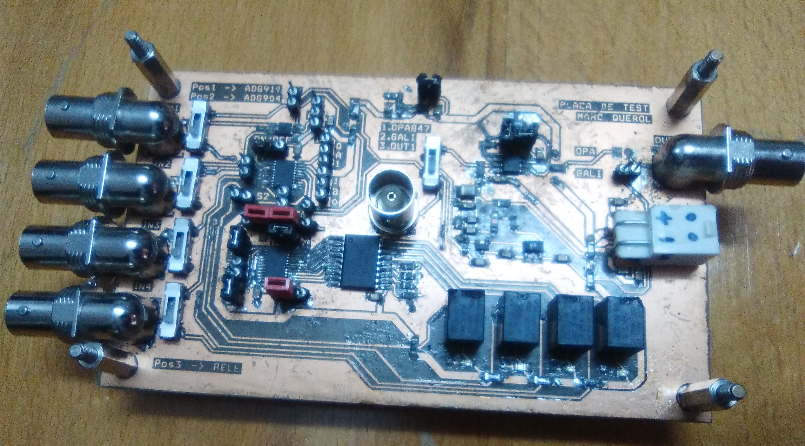
\includegraphics[scale=0.2]{Tarjeta.png} 
}
{
%\subfloat[Espectro de emisión]
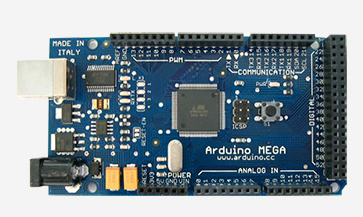
\includegraphics[scale=0.4]{Arduino.png} 
}
\caption{Tarjeta de automatización y Arduino Mega\label{arduino}}
\end{figure} 

Lo más importante de esta tarjeta es que por un lado realiza el proceso de automatización y, por otro, nos permite interaccionar con todas las partes importantes de nuestro experimento, tales como fuente de tensión de alimentación de distintos componentes del sistema, osciloscopios, etc, a partir de un programa llamado LabView.

Como ya se ha mencionado anteriormente esta tarjeta formará parte de un prototipo. El diseño final contendrá un número mucho mayor de bunch de fibras centelleadoras y, por extensión, necesitará un número mayor de SiPM para leer todas estas. Es en este punto cuando cobra una vital importancia el hecho de la automatización tanto en calibración de SiPM como en control de componentes ya que calibrar un número elevado de SiPM (en principio se han previsto 64 SiPM) es un trabajo que llevaría demasiado tiempo. Además, para poder controlar de forma efectiva un número tan elevado de SiPM es necesario un control automático. 

\item {} En cuarto lugar también habrá que proceder a contrucción de un clad para las fibras centelleadoras a partir del proceso de vaporación... en el ICMOL, tema discutido en la sección $\ref{sec:Resultados}$.

\item {} En quinto lugar habrá que conseguir electrónica de bajo ruido en un futuro para poder seguir reduciendo la actividad del prototipo y que podamos distinguir esta señal del fondo.

\item {} En sexto lugar habrá que terminar las simulaciones incluyendo el posterior tratamiento de la luz tras su emisión en las fibras centelleadoras, tema que nos permitirá evaluar la importancia del guiado de luz en las fibras centelleadoras, tema discutido en la sección $\ref{sec:Resultados}$.

\item {} En último lugar se pretende desarrollar un sistema de control de temperatura para disponer de este en el laboratorio de reacciones nucleares. Para ello se contruirá una caja de algún material términcamente asilante, por ejemplo poliespán, en el interior de la cual residirá nuestro foco frío y caliente. El foco frío consistirá en una resistencia térmica unida  a un ventilador de 12V y el foco frío consistirá en un aire acondicionado~\cite{Camara}.

\end{enumerate}